\documentclass[a4paper,12pt,titlepage]{article}
\usepackage{graphicx}



\DeclareGraphicsExtensions{.jpg}
\graphicspath{{./Images/}}

\begin{document}
	\newcommand{\HRule}{\rule{\linewidth}{0.5mm}}
\begin{titlepage}
\begin{center}

\includegraphics[width = 0.3\textwidth]{US_logo.png}~\\[1cm]
\textsc{\LARGE Unsolvable Solutions}\\
Client: Francois Mouton at the CSIR DSSR\\[1.5cm]
\textsc{\Large  Functional Requirements}\\[0.5cm]

 \HRule\\[0.4cm]
{ \huge \bfseries  Eavesdropping Protection in Conclave \\[0.4cm] }

 \HRule\\ 



Github link:  \url{https://github.com/Unsolvable-Solutions/Project-EPIC} \\[1.2cm]

\noindent
\begin{minipage}[t]{0.4\textwidth}

	\begin{flushleft} \large
	\emph{Members:}\\
		Edwin Fullard  \\
		Jaco Bezuidenhoudt \\
		Jandre Coetzee\\
		Maret Stoffberg\\
		Ryno Pierce\\
	\end{flushleft}
\end{minipage}%
\begin{minipage}[t]{0.4\textwidth}
\begin{flushright} \large
	\emph{Student Number:} \\
		12048675 \\
		11013878 \\
		 10693077 \\
		 11071762 \\
		 12003922\\
	\end{flushright}
\end{minipage}

\vfill


% Bottom of the page




\end{center}
\end{titlepage}




	
	% Table of content
	\newpage
	\tableofcontents

\newpage\section{Introduction}
	\subsection{Purpose} The purpose of this Software Design documentation is to introduce and explain to the reader the architecture and designs used in the EPIC project. 

	\subsection{Scope}
This EPIC (Eavesdropping Protection in Conclave) project consist of a server, an Android application and a gateway device. The android device is held over the gateway node and, using NFC, a request to enter the meeting is send to the server via the gateway device. The server then respond with permission or denial. If permission is granted, the android device will proceed into protection mode and the meeting log is updated. After the meeting has been held, the device will then be held over the gateway node again to deactivate the protection mode. A user may query the log of a meeting.
\newline
The eavesdropping malware use a server and an application on the android device. Ideally the application will be hidden behind another application, but for the sake of this project it will be a visible application. A user will send an eavesdropping request from the server to a specified android device. If this device have the malware installed, it will start streaming the recording to the user. The user may then send a request to stop the recording and store the recording.

	\subsection{Overview} This document provides a look at the design of the EPIC project, by the Unsolvable Solutions Team. 

	%\subsection{Reference Material}	

	\subsection{Definitions and Acronyms}
		\begin{itemize}
			\item\textbf{ EPIC} Eavesdropping Protection in Conclave
		\end{itemize}
\newpage\section{System Overview}

 This system consist of two separate parts: the EPIC components and the Eavesdropping Malware software.
\subsection{EPIC}
\begin{figure}[h!]
 			 \centering
			  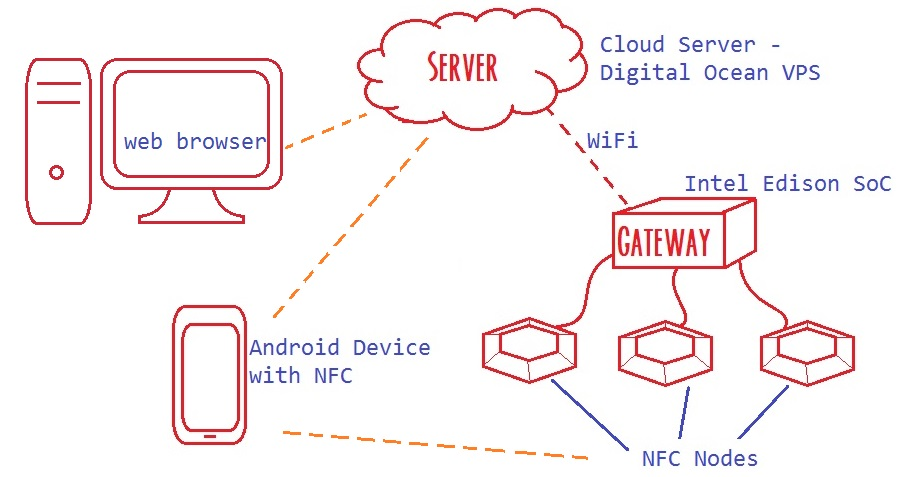
\includegraphics[width=0.8\textwidth]{Overview}
		 	 \caption{Basic representation of the components}
		\end{figure}
Each user is registered with a unique identifier and password on the cloud server. The user may either register via the web browser or when the application is installed. When a meeting is attended, the user hold his Android NFC device over a NFC Node. The device then sends the identifier to the Node via NFC. The Node then sends the users identifier to the gateway to check if the user may enter the meeting. Each gateway is programmed for a specific meeting, and this meeting may only be attended by specified users. If the gateway give the user permission to enter the meeting, the users device is set on silent and the GSM and the Wifi are turned off. The gateway also sends the users identifier and timestamp of entrace to the server. The server keeps a log of all the entries to a meeting. This log may later be viewed via a web browser. The scheduling, updating and deletion of meetings are also done via a browser. After a person is done with the meeting, they scan their device over the NFC Node again, this time the phone is restored to its previous state.
\subsubsection{Eavesdropping Malware Software}


\newpage\section{System Architecture}
	\subsection{Architecture Design}
		\begin{itemize}
			\item\textbf{ Model-View-Controler} This architectural design pattern is used with the server. % ADD MORE HERE
			\item\textbf{ Singleton} The singleton design pattern is used with the Malware. Only one instance of a recoding may happen at a time. % ADD MORE HERE
			\item\textbf{ Singleton} The gateway make use of the Singleton design pattern. There may only be one meeting per gateway. % ADD MORE HERE
		\end{itemize}
	\subsection{Decomposition Description}
	\subsection{Design Rationale}

\newpage\section{Data Design}
	\subsection{Data Description} All the user and meeting data are stored in a MongoDB data structure. % ADD MORE HERE
	\subsection{Data Dictionary}

\newpage\section{Component Design}

\newpage\section{Human Interface Design}
	\subsection{Overview of User Interface}
	\subsection{Screen Images}
	\subsection{Screen Objects and Actions}

	
\newpage\section{Requirements Matrix}
% \newpage\section{Apendices}

\end{document}